\documentclass{beamer}

\usepackage{pgfpages}


\usepackage[utf8]{inputenc}
%\usepackage{xeCJK}
\usepackage{graphicx}
\usepackage {mathtools}
%\usepackage{utopia} %font utopia imported
\usetheme{Ilmenau}


% set colors
\definecolor{myNewColorA}{RGB}{255,103,0} 
\definecolor{myNewColorB}{RGB}{169,169,169} 
\definecolor{myNewColorC}{RGB}{255,103,0} 
\setbeamercolor*{palette primary}{bg=myNewColorC}
\setbeamercolor*{palette secondary}{bg=myNewColorB, fg = white}
\setbeamercolor*{palette tertiary}{bg=myNewColorA, fg = white}
\setbeamercolor*{titlelike}{fg=myNewColorA}
\setbeamercolor*{title}{bg=myNewColorA, fg = white}
\setbeamercolor*{item}{fg=myNewColorA}
\setbeamercolor*{caption name}{fg=myNewColorA}
\usefonttheme{professionalfonts}
\usepackage{natbib}
\usepackage{hyperref}

%------------------------------------------------------------
%\titlegraphic{\includegraphics[height=2cm]{logo.png}} 

\setbeamerfont{title}{size=\large}
\setbeamerfont{subtitle}{size=\small}
\setbeamerfont{author}{size=\small}
\setbeamerfont{date}{size=\small}
\setbeamerfont{institute}{size=\small}
\title{Precios al descubierto: El lado oculto detrás de los alarmantes precios}
\subtitle{Un análisis de los precios en el municipio Habana del Este}
\author{Marian Aguilar Tavier} 

\institute{Universidad de La Habana}
\date[\textcolor{white}{Julio, 2023}]  


\begin{document}
\frame{\titlepage}
\begin{frame}
\frametitle{Contenidos}
\tableofcontents
\end{frame}
%------------------------------------------------------------
\section{Introducción}
    \begin{frame}{Introducción}
 Si alguien decide inmiscuirse dentro de la población cubana para conocer los temas de conversación que usualmente tienen los cubanos, sin importar en qué lugar del territorio nacional se encuentre,  un tema que se destacaría sin duda alguna son los altos precios que tienen los productos que se comercializan en Cuba sin importar su tipo.  Resulta curioso que en muchas ocasiones, para productos de una misma categoría el rango de los precios varía sorprendentemente, pero, ¿existirán verdaderamente factores que determinan el precio de cada producto?
Para darle solución a esta interrogante se ha realizado un estudio de los precios de 5 productos muy consumidos por la población cubana de Habana del Este: la cerveza, el vodka, el whisky, el ron y la cebolla con el objetivo de determinar la existencia o no de factores que influyan en el precio de cada producto.  

    \end{frame}

    \begin{frame}{Procesamiento de los datos}
        \begin{itemize}
            \item Nuestro estudio se centra en el análisis de los precios de en el municipio capitalino de Habana del Este, en el que se recorrieron varios lugares para capturar los datos relacionados con los precios mediante fotos, para luego confeccionar una base de datos mediante un archivo en formato .json teniendo en cuenta una serie da categorías por producto.
            \item Para la manipulación y el procesamiento de los datos utilizamos Python y trabajamos específicamente con la biblioteca Pandas. Luego en el caso de la visualización de los resultados de nuestro análisis utilizamos Matplotlib y Seaborn.
        \end{itemize}
    \end{frame}

\section{Cerveza}
    \begin{frame}{Cerveza por país de exportación}
	    -\small Del análisis de los datos anteriores se comprueba que el país que más importa cerveza en Cuba es España, seguido muy de cerca por Países Bajos, mientras que otros países como China y Polonia se encuentran entre los países con menos exportaciones en el municipio. 
      	\begin{figure}[h]
      	\centering
      	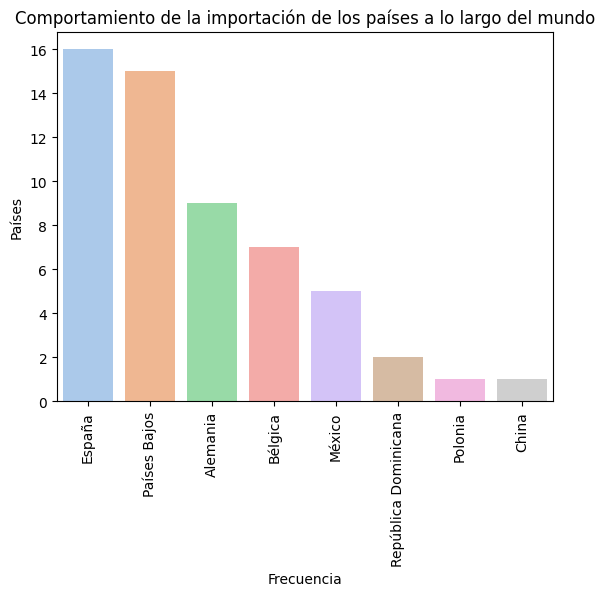
\includegraphics[width=5cm]{export.png}
      \end{figure}
    \end{frame}
    \begin{frame}{Variedades de cerveza por país}
        \small España no solo se encuentra en la cima del top de países que más exportan cerveza, sino que también es el país con más marcas comercializadas en este municipio capitalino con 7 marcas distintas, en segundo lugar se encuentra Países Bajos con 5 marcas de cerveza. En último lugar con respecto a las variedades de cerveza se encuentran nuevamente China, Polonia y República Dominicana.
       \begin{figure}[h]
       	\centering
       	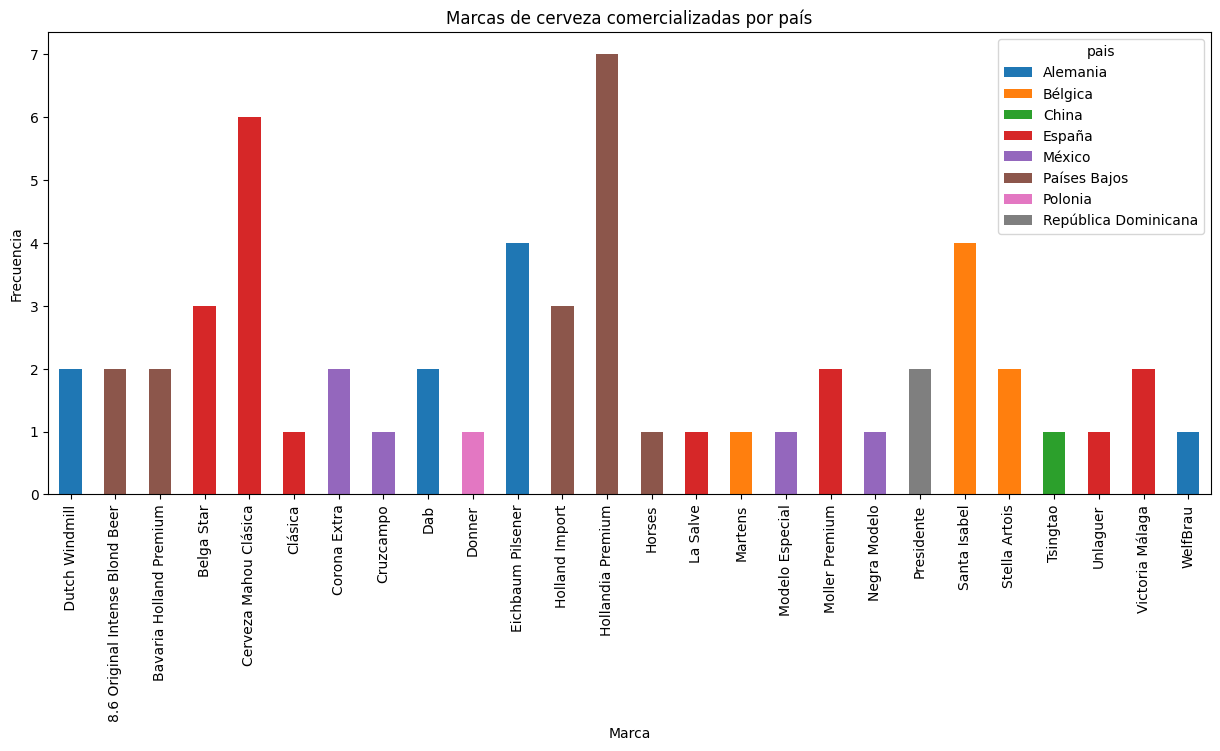
\includegraphics[width=6cm]{country beer.png}
       \end{figure}
        
    \end{frame}
    \begin{frame}{Precio según la marca}
        \small La cerveza más cara es el cerveza WelfBrau, seguida de la Cristal, la Negra Modelo, la Bucanero y la Cristal Extra. De la misma forma las cervezas más económicas que se pueden consumir en esta localidad son la cerveza Clásica, la cerveza Mahou Clásica, la Shekels y la Presidente. 
        \begin{figure}[h]
        	\centering
        	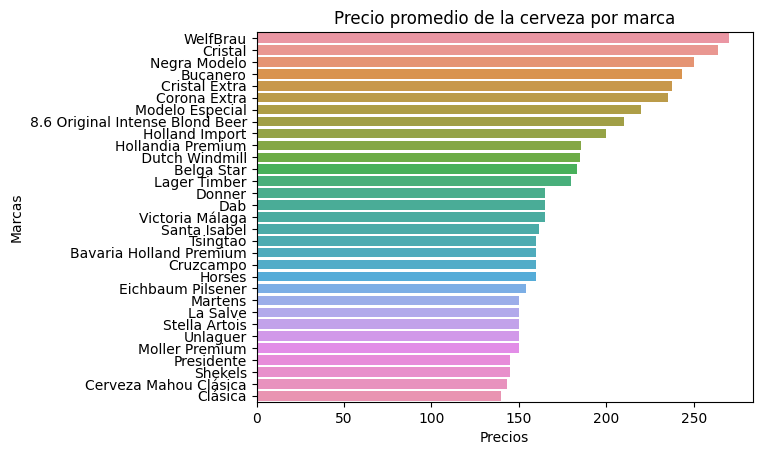
\includegraphics[width=7cm]{price beer.png}
        \end{figure}

    \end{frame}
    \begin{frame}{Otras particularidades observadas}
        \begin{itemize}
    \item En Habana del Este una cerveza tiene un precio promedio de 191 CUP y la cerveza más importada es la Holland Import.
    \item  Se observa además que el consumo de las cervezas claras es mucho mayor al consumo de las cervezas oscuras ya que, el 82.05\% representa a las cervezas claras, mientras que las cervezas oscuras representan solo el 14.10\%.
    \item El precio promedio de una cerveza clara es de 207 CUP, mientras que el de la cerveza oscura es de 188 CUP aproximadamente.
   \end{itemize}

    \end{frame}
    \begin{frame}
     El precio de la cerveza teniendo en cuenta su disponibiliad, no provoca en este caso una diferencia muy notable pues, la cerveza cristal además de ser la más disponible es la más cara, seguida de la Bucanero y en último lugar la Cristal Extra.
     \begin{figure}[h]
     	\centering
     	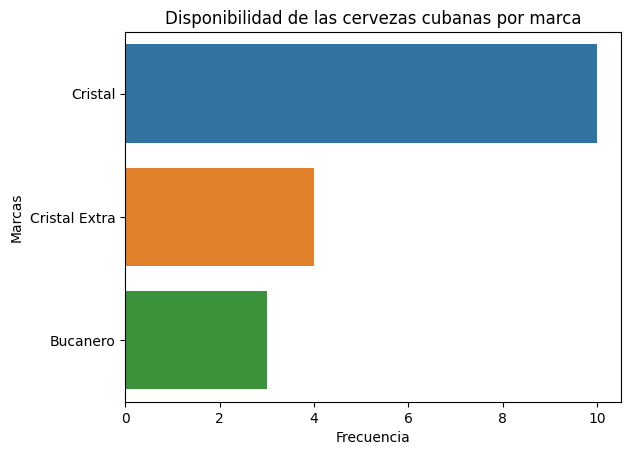
\includegraphics[width=8cm]{cuban beer amount.png}
     \end{figure}

    \end{frame}
\section{Ron}
    \begin{frame}{Precio según material del envase, capacidad y porcentaje de alcohol}
        \begin{itemize}
             \item  El precio promedio de un ron envasado en plástico es de 728 CUP y el precio promedio de una botella de ron de cristal es de 2428.75 CUP.
            \item Si analizamos por otro lado, el porcentaje de alcohol en el caso del ron, una botella de ron en Habana del Este suele encontrarse con un porcentaje de alcohol de 40%.
             \item En cuanto al precio según la capacidad, el precio promedio de una botella de ron de 750 mililitros es de 1100 CUP, el precio promedio de una botella de 1000 ml es de 1517 CUP aproximadamente.
        \end{itemize}

    \end{frame}
    \begin{frame}{Precio por marca}
        En este caso los rones que presentan mayor disponibilidad se encuentran en el rango intermedio de precios. Mientras que los rones más caros son el Havana Club Selección de Maestros, el Ron Santiago de Cuba 11 Años y el Pacto Navío.
        \begin{figure}[h]
        	\centering
        	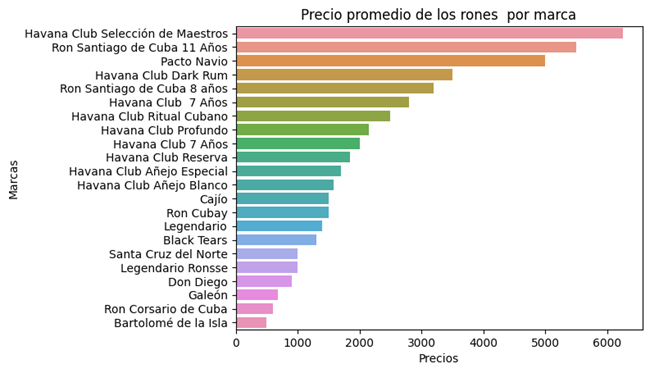
\includegraphics[width=8cm]{rum prices.png}
        \end{figure}

    \end{frame}

\section{Whisky}
    \begin{frame}{Particularidades del producto}
      \small En cuanto a las marcas de whisky la que más se exporta en este municipio es el whisky Chanceler, seguido del Old Partner y el Chanceler Edición Especial. Se observa además que Brasil, que es el país que representa al whisky más importado no coincide con el país que más importa whisky, ya que este lugar está ocupado por Escocia. 
     \begin{figure}[h]
     	\centering
     	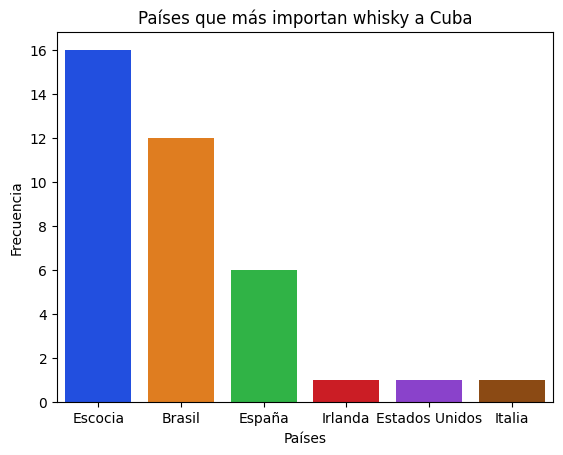
\includegraphics[width=5cm]{whisky export.png}
     \end{figure}

    \end{frame}
\section{Vodka}
    \begin{frame}{Particularidades del producto}
         \begin{itemize}
             \item El vodka más importado en este caso es el de la marca Tabarish, el cual es un vodka ruso.
             \item  El porcentaje de alcohol más común que se encuentra en una botella es de 40\% de alcohol.
             \item El Vodka Krilof Black, tiene un porcentaje de alcohol de  20\%, sin embargo cabe destacar que aunque este porcentaje está  por debajo del promedio, continúa siendo una gran amenaza para la salud humana.
         \end{itemize}.

    \end{frame}
    \begin{frame}{Comparación de los tres productos}
       \small Analizando los precios de los tres productos anteriores, comprobamos que una botella de ron tiene un precio promedio de 2161 CUP, el whisky 2801 CUP, mientras el precio del vodka es de 1964 CUP.

        \begin{figure}[h]
       	\centering
       	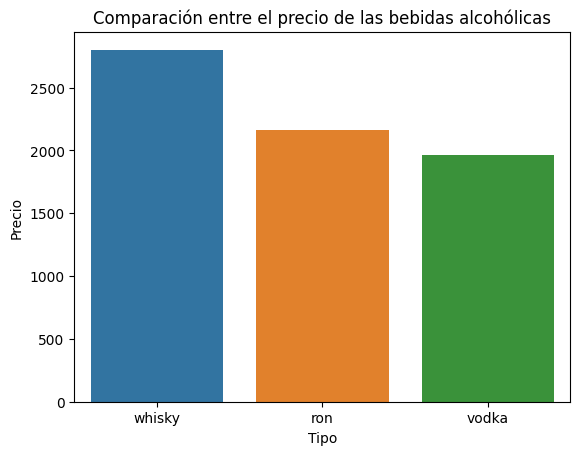
\includegraphics[width=7cm]{comparation.png}
       \end{figure}

    \end{frame}
 \section{Cebolla}
    \begin{frame}{Particularidades de la cebolla}
         \small Al analizar el precio de a cebolla según su color, los resultados arrojan a que la diferencia de precio atendiendo al color de la cebolla es muy pequeña. Mientras que el precio promedio de la cebolla blanca es de aproximadamente 164 CUP, el de la cebolla morada es de 154 CUP.
        \begin{figure}[h]
       	\centering
       	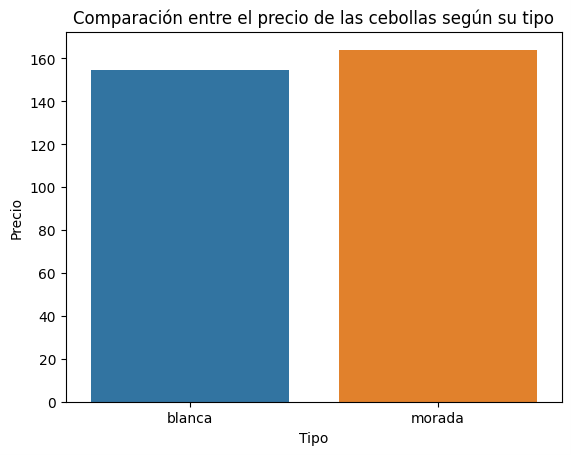
\includegraphics[width=6cm]{onion.png}
       \end{figure}

    \end{frame}

\section{Conclusiones}
    \begin{frame}{Conclusiones}
        \begin{itemize}
        \item El factor precio se ve influenciado por una serie de elementos, que a la vez varían en dependencia del producto.
        \item Es importante mencionar que nuestro estudio de los precios está comprendido entre los meses de abril y mayo del año 2023. Por lo que puede ser utilizado posteriormente para el análisis de los precios de estos productos en años posteriores para así analizar su variación a lo largo del tiempo. 
        \end{itemize}
    \end{frame}



\end{document}




